\documentclass[9pt,mathserif,aspectratio=169]{beamer}
\usepackage[utf8]{inputenc} %Some citations and accents need this

%\useoutertheme{smoothbars} %Disabled: too many sections causes header overflow
\setbeamertemplate{headline}{} %Clean header -- no navigation bar
\usetheme{Dal_4x3}
\usecolortheme{Dal}

\usepackage{transparent} % \transparent{0.3}{ <stuff> } will make that stuff have 30% opacity.
\usepackage{changepage} % \begin{adjustwidth}{+50pt}{-200pt} will add 50pt to left margin, take 200pt from right

\usepackage{upgreek} %To get \uppi
	\renewcommand{\pi}{\uppi}
	\newcommand{\e}{\mathrm{e}} %Exponential
	\renewcommand{\i}{\mathrm{i}} %Imaginary Number
\usepackage{bm} %Very outdated package that still works for bolding greek letters.
\usepackage{pifont}% For checkmarks and x's
	\newcommand{\cmark}{\ding{51}}%
	\newcommand{\xmark}{\ding{55}}%

\usepackage{tcolorbox}
\usepackage{braket}
\usepackage{bm} %Bold math \bm and \boldsymbol
	\newcommand{\bs}{\boldsymbol}
\usepackage{animate} %Alternate for animations
\usepackage{verbatim}
\usepackage{chemformula} %\ch{H2}
\usepackage{listings}
\usepackage{ragged2e} %For \justifying
\usepackage{physics} %Adds \abs{} for absolute value brackets, and other physics related commands
\usepackage{braket} %Adds \braket{0|0}, \bra{0}, or \ket{0}
\usepackage{ulem}
\usepackage[hang,flushmargin]{footmisc} %To remove indent from footnote
\usepackage{caption, subcaption} %Adds \begin{subfigure}{0.5\textwidth}{} \caption{}... to existing figures.
\usepackage{parskip}
	\setlength{\parskip}{\smallskipamount}
	\setlength{\parindent}{0pt}
\usepackage{appendixnumberbeamer}


\usepackage{amstext} 	% for \text macro
\usepackage{array}	 	% for \newcolumntype macro
\usepackage{booktabs}	% for \toprule \midrule \bottomrule in tables
	\newcolumntype{L}{>{$}l<{$}} % math-mode version of "l" column type
	\newcolumntype{C}{>{$}c<{$}} % math-mode version of "c" column type
	\newcolumntype{R}{>{$}r<{$}} % math-mode version of "r" column type



%%%%%%%%%%%%%%%%%% for \rowcolor
\usepackage{xcolor,colortbl}
%%%%%%%%%%%%%%%%%%


%Write Fortran code with syntax highlighting
\definecolor{snow}{rgb}{1.0, 0.98, 0.98}
\definecolor{lavendergray}{rgb}{0.77, 0.76, 0.82}
\definecolor{charcoal}{rgb}{0.21, 0.27, 0.31}
\definecolor{black}{rgb}{0.0, 0.0, 0.0}
\definecolor{huntergreen}{rgb}{0.21, 0.37, 0.23}
\definecolor{burntorange}{rgb}{0.8, 0.33, 0.0}
\definecolor{darkred}{rgb}{0.55, 0.0, 0.0}
\lstset{
	language=Fortran,
    backgroundcolor=\color{snow},
    numberstyle=\small\color{lavendergray},
    commentstyle=\color{charcoal},
    identifierstyle=\color{black},
    stringstyle=\color{huntergreen},
    keywordstyle=\bfseries\color{burntorange},
    basicstyle=\scriptsize\ttfamily,
    breakatwhitespace=false,
    breaklines=true,
    captionpos=b,
    keepspaces=true,
    numbers=left,
    numbersep=5pt,
    showspaces=false,
    showstringspaces=false,
    showtabs=false,
    tabsize=2
}

%textpos already loaded by theme
\newcommand{\source}[1]{\begin{textblock*}{12cm}(0.5cm,8.5cm)
    \begin{beamercolorbox}[ht=0.2cm,left]{framesource}
        \usebeamerfont{framesource}\usebeamercolor[fg]{framesource} {#1}
    \end{beamercolorbox}
\end{textblock*}}
%\setbeamercolor{framesource}{fg=gray}
\setbeamerfont{framesource}{size=\tiny}


%Uncovering graphics with transparency
\newcommand<>{\uncovergraphics}[2][{}]{
    % Taken from: <https://tex.stackexchange.com/a/354033/95423>
    \begin{tikzpicture}
    \node[anchor=south west,inner sep=0] (B) at (4,0)
        {\includegraphics[#1]{#2}};
    \alt#3{}{%
        \fill [draw=none, fill=white, fill opacity=0.7] (B.north west) -- (B.north east) -- (B.south east) -- (B.south west) -- (B.north west) -- cycle;
    }
    \end{tikzpicture}
}

%doi command for auto-hyperlinking references
\newcommand*{\doi}[1]{\href{http://dx.doi.org/#1}{doi: #1}}



\newtheorem{mybox}{}
\definecolor{red4}{rgb}{0.55, 0.0, 0.0}
\newcommand{\emphr}[1]{{\color{red4}\it\bfseries #1}}

\setbeamerfont{page number in head/foot}{size=\tiny}
\setbeamertemplate{footline}[frame number]

\title[CHM328 -- DFT Lecture 2]{
\centering
\vspace*{1.75cm}\\
\textsc{
	\LARGE Density Functional Theory:\\
	Transition States, Reaction Mechanisms,\\
	and Energy Profiles\\
}
\vspace*{2ex}
\href{https://github.com/albdprice}{\includegraphics[height=0.25\textheight]{chem.jpeg}}\\
\vspace*{1ex}
\Large Alastair J. Price\\
\normalsize \textit{Guest Lecturer}\\
\vspace*{1ex}
\normalsize CHM328H1 S -- Modern Physical Chemistry\\
\normalsize University of Toronto -- Winter 2026
}

\begin{document}

% ============================================================================
% TITLE
% ============================================================================
\section{Introduction}
\begin{frame}[plain]
  \titlepage
\end{frame}

% ============================================================================
% RECAP & OUTLINE
% ============================================================================
\begin{frame}{Recap from Lecture 1}
\begin{columns}
\begin{column}{0.48\textwidth}
\textbf{What we covered:}
\begin{itemize}
\item Molecular Hamiltonian \& Born--Oppenheimer approximation
\item HF theory vs.\ DFT
\item Kohn--Sham DFT and $E_\text{XC}$
\item Jacob's ladder of functionals
\item Potential energy surface (PES)
\item Harmonic approximation \& normal modes
\item Partition functions from DFT
\item Thermodynamic properties ($\Delta G$, $\Delta H$, $\Delta S$)
\end{itemize}
\end{column}
\begin{column}{0.48\textwidth}
\textbf{Key result:}
\[
G = E_\text{elec} + E_\text{ZPE} + H_\text{thermal} - TS
\]

\vspace{0.5em}
\textbf{Today:}\\
How do we use DFT to study \emphr{chemical reactions}?\\
\small\textit{(Recall Week 1: thermo is empirical. DFT makes it predictive.)}
\begin{itemize}
\item Finding transition states
\item Building reaction energy profiles
\item Computing rate constants
\item Understanding selectivity
\end{itemize}
\end{column}
\end{columns}
\end{frame}

\begin{frame}{Lecture 2 Overview}
\begin{columns}
\begin{column}{0.48\textwidth}
\textbf{Part I: Transition State Theory}
\begin{enumerate}
\item Transition states on the PES
\item Saddle points \& imaginary frequencies
\item Transition state theory (TST)
\item The Eyring equation
\item Thermodynamic activation parameters
\end{enumerate}
\end{column}
\begin{column}{0.48\textwidth}
\textbf{Part II: Computational Practice}
\begin{enumerate}
\setcounter{enumi}{5}
\item Finding transition states computationally
\item Intrinsic reaction coordinate (IRC)
\item Building reaction energy profiles
\item Selectivity and competing pathways
\item Case studies in organic \& inorganic chemistry
\end{enumerate}
\end{column}
\end{columns}
\vfill
\begin{center}
\small \textit{Goal: Learn how to use DFT to compute reaction barriers, rate constants,\\and predict which products form and why.}
\end{center}
\end{frame}


% ============================================================================
% SECTION 1: TRANSITION STATES ON THE PES
% ============================================================================
\section{Transition States on the PES}

\begin{frame}{Chemical Reactions on the PES}
\begin{columns}
\begin{column}{0.50\textwidth}
\centering
\includegraphics[width=\textwidth]{PES.png}
\end{column}
\begin{column}{0.48\textwidth}
A chemical reaction is a path on the PES from \textbf{reactant minimum} to \textbf{product minimum}.

\vspace{0.5em}
\textbf{Key features:}
\begin{itemize}
\item \textbf{Minima}: stable species (reactants, products, intermediates)
\item \textbf{Saddle points}: \emphr{transition states} (TS) -- highest point along the minimum energy path
\item \textbf{Reaction coordinate}: the path connecting R $\rightarrow$ TS $\rightarrow$ P
\end{itemize}

\vspace{0.5em}
The \textbf{activation energy} $E_a$ is the energy difference between the TS and reactants.

\vspace{0.3em}
\small\textit{Recall the curse of dimensionality from Week 3: $\sim\!10^{3N-6}$ grid points on the PES. Finding a TS on this surface is the challenge we tackle today.}
\end{column}
\end{columns}
\end{frame}

\begin{frame}{What is a Transition State?}
\begin{tcolorbox}[colback=blue!5!white,colframe=blue!50!black,title=Definition]
A \textbf{transition state} (TS) is a first-order saddle point on the PES:\\
-- a \emphr{maximum} along the reaction coordinate\\
-- a \emphr{minimum} in all other directions
\end{tcolorbox}

\vspace{0.5em}
\textbf{Mathematical characterization:}
\begin{itemize}
\item $\nabla E = \mathbf{0}$ \quad (stationary point, like a minimum)
\item Hessian has \emphr{exactly one negative eigenvalue}
\item $\Rightarrow$ exactly \emphr{one imaginary frequency}
\item The eigenvector of the imaginary frequency shows the \emphr{reaction coordinate} -- the motion that converts reactants to products
\end{itemize}

\vspace{0.5em}
\begin{center}
\begin{tabular}{lcc}
\toprule
& \textbf{Minimum} & \textbf{Transition State} \\
\midrule
Gradient & $\mathbf{0}$ & $\mathbf{0}$ \\
Hessian eigenvalues & All positive & One negative \\
Imaginary frequencies & 0 & \emphr{1} \\
\bottomrule
\end{tabular}
\end{center}
\end{frame}

\begin{frame}{Imaginary Frequencies -- The Signature of a TS}
\centering
\includegraphics[width=0.55\textwidth]{Frequencies.png}

\vspace{0.5em}
\begin{columns}
\begin{column}{0.48\textwidth}
\textbf{At a minimum:}
\begin{itemize}
\item All frequencies are \textbf{real} (positive)
\item All Hessian eigenvalues $> 0$
\item The structure is a \textbf{stable} species
\end{itemize}
\end{column}
\begin{column}{0.48\textwidth}
\textbf{At a transition state:}
\begin{itemize}
\item One frequency is \textbf{imaginary} ($i\nu$)
\item One Hessian eigenvalue $< 0$
\item The mode shows \emphr{bond breaking/forming}
\end{itemize}
\end{column}
\end{columns}

\vspace{0.5em}
\textbf{Always verify your TS:} visualize the imaginary mode -- does it correspond to the reaction you expect?
\end{frame}

\begin{frame}{The Reaction Coordinate}
\begin{columns}
\begin{column}{0.45\textwidth}
\centering
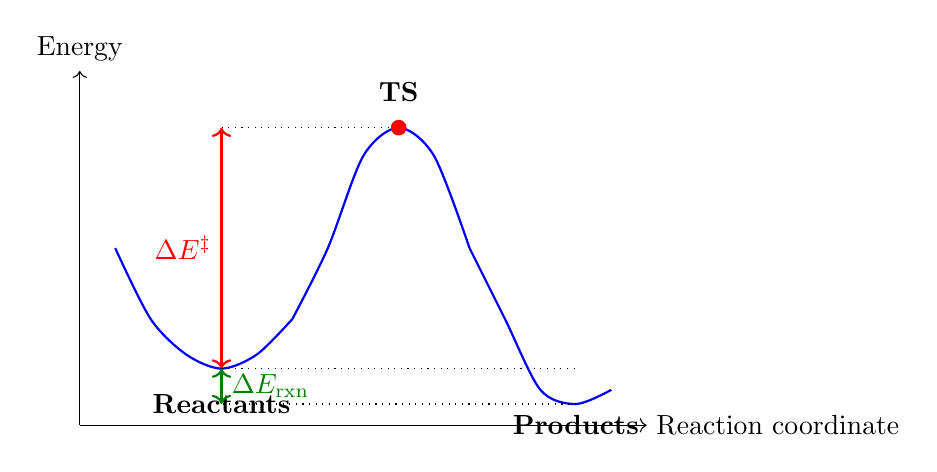
\begin{tikzpicture}[scale=0.90]
\draw[->] (0,0) -- (8,0) node[right] {Reaction coordinate};
\draw[->] (0,0) -- (0,5) node[above] {Energy};
% Reactant well
\draw[thick,blue,smooth] plot coordinates {(0.5,2.5) (1,1.5) (1.5,1) (2,0.8) (2.5,1) (3,1.5)};
% Barrier
\draw[thick,blue,smooth] plot coordinates {(3,1.5) (3.5,2.5) (4,3.8) (4.5,4.2) (5,3.8) (5.5,2.5)};
% Product well
\draw[thick,blue,smooth] plot coordinates {(5.5,2.5) (6,1.5) (6.5,0.5) (7,0.3) (7.5,0.5)};
% Labels
\node at (2,0.3) {\textbf{Reactants}};
\node at (4.5,4.7) {\textbf{TS}};
\node at (7,0) {\textbf{Products}};
% Arrows
\draw[<->,thick,red] (2,0.8) -- node[left] {$\Delta E^\ddagger$} (2,4.2);
\draw[<->,thick,green!50!black] (2,0.8) -- node[right] {$\Delta E_\text{rxn}$} (2,0.3);
\draw[dotted] (2,0.8) -- (7,0.8);
\draw[dotted] (2,4.2) -- (4.5,4.2);
\draw[dotted] (7,0.3) -- (2,0.3);
% TS marker
\node[circle,fill=red,inner sep=2pt] at (4.5,4.2) {};
\end{tikzpicture}
\end{column}
\begin{column}{0.51\textwidth}
\small
\textbf{Energy profile:}
\begin{itemize}
\setlength\itemsep{0.05em}
\item $\Delta E^\ddagger$ = activation energy
\item $\Delta E_\text{rxn}$ = reaction energy
\end{itemize}

\vspace{-0.3em}
\textbf{Hammond's postulate:}\\
\vspace{0.1em}
Exothermic $\Rightarrow$ TS resembles reactants\\
Endothermic $\Rightarrow$ TS resembles products
\end{column}
\end{columns}
\end{frame}

\begin{frame}{Multi-Step Reactions}
Many reactions proceed through \emphr{intermediates}:

\vspace{0.2em}
\centering
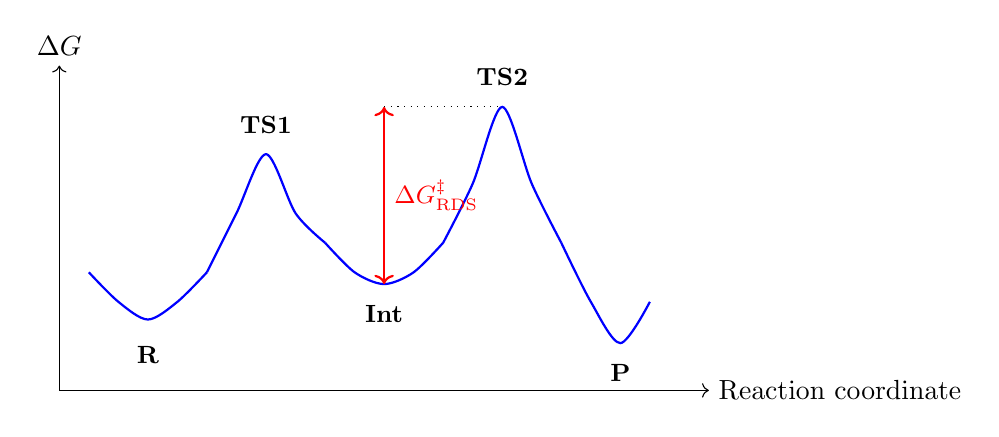
\begin{tikzpicture}[scale=0.75]
\draw[->] (0,0) -- (11,0) node[right] {Reaction coordinate};
\draw[->] (0,0) -- (0,5.5) node[above] {$\Delta G$};
% Reactant
\draw[thick,blue,smooth] plot coordinates {(0.5,2) (1,1.5) (1.5,1.2) (2,1.5) (2.5,2)};
% TS1
\draw[thick,blue,smooth] plot coordinates {(2.5,2) (3,3) (3.5,4) (4,3) (4.5,2.5)};
% Intermediate
\draw[thick,blue,smooth] plot coordinates {(4.5,2.5) (5,2.0) (5.5,1.8) (6,2.0) (6.5,2.5)};
% TS2
\draw[thick,blue,smooth] plot coordinates {(6.5,2.5) (7,3.5) (7.5,4.8) (8,3.5) (8.5,2.5)};
% Product
\draw[thick,blue,smooth] plot coordinates {(8.5,2.5) (9,1.5) (9.5,0.8) (10,1.5)};
% Labels
\node at (1.5,0.6) {\small\textbf{R}};
\node at (3.5,4.5) {\small\textbf{TS1}};
\node at (5.5,1.3) {\small\textbf{Int}};
\node at (7.5,5.3) {\small\textbf{TS2}};
\node at (9.5,0.3) {\small\textbf{P}};
% Rate-determining step
\draw[<->,thick,red] (5.5,1.8) -- node[right] {\small $\Delta G^\ddagger_\text{RDS}$} (5.5,4.8);
\draw[dotted] (5.5,4.8) -- (7.5,4.8);
\end{tikzpicture}

\vspace{0.5em}
\begin{itemize}
\item The \textbf{rate-determining step (RDS)} has the \emphr{highest barrier} relative to the lowest preceding intermediate
\item All minima and TS must be optimized and characterized by frequency calculations
\item The overall barrier is from the \emphr{resting state} to the \emphr{highest TS}
\end{itemize}
\end{frame}


% ============================================================================
% SECTION 2: TRANSITION STATE THEORY
% ============================================================================
\section{Transition State Theory}

\begin{frame}{Transition State Theory (TST) -- Assumptions}
\textbf{Eyring's TST} (1935) connects the microscopic PES to macroscopic rate constants:

\vspace{0.5em}
\textbf{Key assumptions:}
\begin{enumerate}
\item The Born--Oppenheimer approximation is valid
\item Classical nuclear motion along the reaction coordinate
\item \textbf{Quasi-equilibrium:} Reactants and the TS are in quasi-thermodynamic equilibrium:
\[
\ch{A + B} \rightleftharpoons [\ch{AB}]^\ddagger \rightarrow \text{Products}
\]
\item The TS is crossed only once (no re-crossing)
\item Separability of the reaction coordinate from other degrees of freedom
\end{enumerate}

\vspace{0.5em}
\textbf{TST provides an \emphr{upper bound} to the true rate constant} (re-crossing lowers the rate).
\end{frame}

\begin{frame}{The Eyring Equation}
\begin{tcolorbox}[colback=green!5!white,colframe=green!50!black,title=The Eyring Equation]
\[
\boxed{k(T) = \kappa \frac{k_BT}{h}\e^{-\Delta G^\ddagger / RT}}
\]
\end{tcolorbox}

\vspace{0.5em}
\begin{itemize}
\item $k(T)$ = rate constant at temperature $T$
\item $\kappa$ = transmission coefficient ($\leq 1$, often assumed $= 1$)
\item $k_B T / h$ = frequency factor ($\approx 6.2 \times 10^{12}$ s$^{-1}$ at 298 K)
\item $\Delta G^\ddagger$ = Gibbs free energy of activation
\end{itemize}

\vspace{0.5em}
\textbf{Alternatively}, in terms of $\Delta H^\ddagger$ and $\Delta S^\ddagger$:
\[
k(T) = \kappa \frac{k_BT}{h}\e^{\Delta S^\ddagger / R}\e^{-\Delta H^\ddagger / RT}
\]

\vspace{0.3em}
\small Compare with Arrhenius: $k = A\e^{-E_a/RT}$ \quad $\Rightarrow$ \quad $E_a \approx \Delta H^\ddagger + RT$

\vspace{0.3em}
\small\textit{The $\Delta G^\ddagger$ here is computed from the same $q_\text{trans} \cdot q_\text{rot} \cdot q_\text{vib} \cdot q_\text{elec}$ partition function machinery you've been building all term --- now applied to the TS.}
\end{frame}

\begin{frame}{Activation Parameters from DFT}
\textbf{From DFT frequency calculations on reactants and TS:}

\begin{align*}
\Delta E^\ddagger &= E_\text{elec}(\text{TS}) - E_\text{elec}(\text{R}) & \text{electronic barrier} \\[4pt]
\Delta E_0^\ddagger &= \Delta E^\ddagger + \Delta E_\text{ZPE}^\ddagger & \text{ZPE-corrected barrier} \\[4pt]
\Delta H^\ddagger &= \Delta E_0^\ddagger + \Delta H_\text{thermal}^\ddagger & \text{enthalpy of activation} \\[4pt]
\Delta G^\ddagger &= \Delta H^\ddagger - T\Delta S^\ddagger & \text{free energy of activation}
\end{align*}

\vspace{0.5em}
\begin{tcolorbox}[colback=yellow!5!white,colframe=yellow!50!black]
\textbf{Important:} The TS has $3M-7$ real vibrational modes (one mode is the reaction coordinate and is \emphr{excluded} from $q_\text{vib}^\ddagger$). This is already handled automatically by the frequency calculation!
\end{tcolorbox}
\end{frame}

\begin{frame}{Deriving the Eyring Equation}
\textbf{Starting from TST quasi-equilibrium:}
\[
K^\ddagger = \frac{[\text{TS}]}{[\text{R}]} = \frac{q^\ddagger}{q_\text{R}} \e^{-\Delta E_0^\ddagger / k_BT}
\]

\vspace{0.3em}
The TS partition function is factored:
\[
q^\ddagger = \underbrace{q^\ddagger_\text{react.\ coord.}}_{\text{1D translation}} \times q^\ddagger_\text{remaining}
\]

The reaction coordinate contribution (particle in a box of width $\delta$):
\[
q^\ddagger_\text{react.\ coord.} = \frac{\sqrt{2\pi \mu k_B T}}{h}\,\delta
\]

The rate of crossing the barrier:
\[
k = \frac{k_BT}{h} \cdot \frac{q^\ddagger_\text{remaining}}{q_\text{R}} \cdot \e^{-\Delta E_0^\ddagger / k_BT} = \frac{k_BT}{h}\,K^\ddagger_\text{thermo} = \frac{k_BT}{h}\e^{-\Delta G^\ddagger/RT}
\]
\end{frame}

\begin{frame}{Numerical Example: How Barrier Height Affects Rate}
Using the Eyring equation at $T = 298$ K:
\[
k = \frac{k_BT}{h}\e^{-\Delta G^\ddagger / RT} \approx 6.2 \times 10^{12} \cdot \e^{-\Delta G^\ddagger / RT} \;\; \text{s}^{-1}
\]

\vspace{0.5em}
\begin{center}
\begin{tabular}{ccc}
\toprule
$\Delta G^\ddagger$ (kcal/mol) & $k$ (s$^{-1}$) & \textbf{Half-life} \\
\midrule
5 & $1.4 \times 10^{9}$ & $\sim$0.5 ns \\
10 & $3.1 \times 10^{5}$ & $\sim$2 $\mu$s \\
15 & $6.8 \times 10^{1}$ & $\sim$10 ms \\
\rowcolor{yellow!20} 20 & $1.5 \times 10^{-2}$ & $\sim$46 s \\
25 & $3.3 \times 10^{-6}$ & $\sim$2.4 days \\
30 & $7.3 \times 10^{-10}$ & $\sim$30 years \\
35 & $1.6 \times 10^{-13}$ & $\sim$140{,}000 years \\
\bottomrule
\end{tabular}
\end{center}

\vspace{0.3em}
\emphr{1 kcal/mol error in $\Delta G^\ddagger$} changes the rate by a factor of $\sim$5.5!\\
\small This is why accurate barriers are so important (and challenging).
\end{frame}

\begin{frame}{Reaction Path Degeneracy}
\textbf{If there are $\sigma_\text{rxn}$ equivalent pathways}, the rate is multiplied:
\[
k_\text{obs} = \sigma_\text{rxn} \cdot k_\text{single path}
\]

\vspace{0.5em}
\textbf{Examples:}
\begin{itemize}
\item \textbf{H-abstraction from \ch{CH4}:} 4 equivalent C--H bonds $\Rightarrow$ $\sigma_\text{rxn} = 4$
\item \textbf{Deprotonation of \ch{C2H6}:} 6 equivalent C--H bonds $\Rightarrow$ $\sigma_\text{rxn} = 6$
\item \textbf{S\textsubscript{N}2 at \ch{CH3Cl}:} only 1 backside attack $\Rightarrow$ $\sigma_\text{rxn} = 1$
\end{itemize}

\vspace{0.5em}
\begin{tcolorbox}[colback=blue!5!white,colframe=blue!50!black]
$\sigma_\text{rxn} = \dfrac{\sigma_\text{R}}{\sigma_\text{TS}}$, where $\sigma$ are the rotational symmetry numbers.

\vspace{0.3em}
This accounts for the fact that symmetry-equivalent paths are already included in the rotational partition functions.
\end{tcolorbox}
\end{frame}


% ============================================================================
% SECTION 3: FINDING TRANSITION STATES
% ============================================================================
\section{Finding Transition States}

\begin{frame}{TS Optimization -- The Challenge}
\begin{columns}
\begin{column}{0.55\textwidth}
Finding a TS is \emphr{much harder} than finding a minimum:

\vspace{0.5em}
\begin{itemize}
\item A minimum is a ``bowl'' -- optimization naturally rolls downhill
\item A TS is a ``saddle'' -- must go \emphr{uphill} along reaction coordinate and \emphr{downhill} in all others
\item No guarantee of finding the \emphr{right} TS
\item Multiple TS may exist for the same reaction
\item Requires a \textbf{good initial guess}
\end{itemize}
\end{column}
\begin{column}{0.42\textwidth}
\centering
\begin{tikzpicture}[scale=0.8]
% Saddle surface
\draw[thick,->] (0,0,0) -- (5,0,0) node[right] {$x$};
\draw[thick,->] (0,0,0) -- (0,4,0) node[above] {$E$};
\draw[thick,->] (0,0,0) -- (0,0,4) node[below left] {$y$};
% Saddle point
\node[circle,fill=red,inner sep=2pt] at (2.5,2,2) {};
\node[above right] at (2.5,2.2,2) {\textbf{TS}};
% Arrows showing up/down directions
\draw[->,thick,blue] (2.5,2,2) -- (2.5,3,2) node[right] {\small max};
\draw[->,thick,green!50!black] (2.5,2,2) -- (2.5,1,2);
\draw[->,thick,red] (2.5,2,0.5) -- (2.5,2,2);
\draw[->,thick,red] (2.5,2,3.5) -- (2.5,2,2);
\node[below,red] at (2.5,1.5,0.5) {\small min};
\end{tikzpicture}

\vspace{0.5em}
\small Saddle point: maximum in one direction, minimum in all others.
\end{column}
\end{columns}
\end{frame}

\begin{frame}{Method 1: Relaxed PES Scan}
\textbf{Approach:} Systematically vary the reaction coordinate while optimizing all other coordinates.

\vspace{0.5em}
\textbf{Procedure:}
\begin{enumerate}
\item Choose a coordinate that changes during the reaction (e.g., a bond length)
\item Fix this coordinate at a series of values between reactant and product
\item At each point, optimize all other coordinates (``relaxed scan'')
\item The maximum of the scan gives an \textbf{approximate TS geometry}
\item Use this as the starting point for a proper TS optimization
\end{enumerate}

\vspace{0.5em}
\textbf{Advantages:}
\begin{itemize}
\item Gives a visual picture of the reaction path
\item Helps identify the right reaction coordinate
\item Good for generating TS guesses
\end{itemize}

\vspace{0.3em}
\textbf{Limitation:} The scan coordinate may not be the true reaction coordinate.
\end{frame}

\begin{frame}{Method 2: QST2 and QST3}
\textbf{Quadratic Synchronous Transit} -- uses knowledge of reactant and product geometries:

\vspace{0.5em}
\textbf{QST2:} Requires reactant + product geometries
\begin{itemize}
\item Interpolates a path and finds the maximum along it
\item Then refines using eigenvector-following
\end{itemize}

\vspace{0.5em}
\textbf{QST3:} Requires reactant + TS guess + product geometries
\begin{itemize}
\item Better convergence with a reasonable TS guess
\item The TS guess can come from a relaxed scan
\end{itemize}

\vspace{0.5em}
\begin{tcolorbox}[colback=yellow!5!white,colframe=yellow!50!black]
\textbf{Critical:} Atom ordering must be \emphr{consistent} between reactant, TS, and product structures! The algorithm maps atoms by index.
\end{tcolorbox}

\vspace{0.3em}
In Gaussian: \texttt{opt=(QST2)} or \texttt{opt=(QST3)}\\
In ORCA: \texttt{NEB-TS} (nudged elastic band $\rightarrow$ TS)
\end{frame}

\begin{frame}{Method 3: Nudged Elastic Band (NEB)}
\textbf{NEB} finds the \textbf{minimum energy path (MEP)} between two endpoints:

\vspace{0.5em}
\begin{enumerate}
\item Generate a ``chain'' of images (structures) between reactant and product
\item Connect images with ``springs'' (elastic band)
\item Optimize the band: minimize perpendicular forces, maintain spacing
\item The highest-energy image approximates the TS
\end{enumerate}

\vspace{0.5em}
\textbf{Climbing-Image NEB (CI-NEB):}
\begin{itemize}
\item The highest image is driven \emphr{uphill} along the path
\item Converges to the true saddle point
\end{itemize}

\vspace{0.5em}
\textbf{Advantages:}
\begin{itemize}
\item Does not require a TS guess
\item Finds the MEP, not just the TS
\item Good for complex reactions where the coordinate is unclear
\end{itemize}

\textbf{Disadvantage:} Computationally expensive (many images, many optimizations)
\end{frame}

\begin{frame}{Method 4: Eigenvector Following (Berny Algorithm)}
\textbf{Direct TS optimization:} Follow the lowest eigenvector of the Hessian uphill.

\vspace{0.5em}
\textbf{Procedure:}
\begin{enumerate}
\item Start with a TS guess (from scan, NEB, or chemical intuition)
\item Compute or estimate the Hessian
\item Maximize along the eigenvector with the \emphr{most negative} eigenvalue
\item Minimize along all other eigenvectors
\item Iterate until convergence
\end{enumerate}

\vspace{0.5em}
\textbf{In Gaussian:} \texttt{opt=(TS,CalcFC)} or \texttt{opt=(TS,CalcAll)}
\begin{itemize}
\item \texttt{CalcFC}: compute the Hessian at the first step
\item \texttt{CalcAll}: compute the Hessian at every step (expensive but reliable)
\end{itemize}

\vspace{0.5em}
\begin{tcolorbox}[colback=red!5!white,colframe=red!50!black]
\textbf{Warning:} The initial guess \emphr{must} already be close to the TS! The algorithm follows the \emphr{nearest} saddle point, which may not be the one you want.
\end{tcolorbox}
\end{frame}

\begin{frame}{Verifying the Transition State}
\textbf{After finding a TS, you MUST verify it:}

\vspace{0.5em}
\begin{enumerate}
\item \textbf{Frequency calculation:} Confirm exactly \emphr{one imaginary frequency}
\begin{itemize}
\item Zero imaginary $\rightarrow$ it's a minimum, not a TS!
\item Two or more $\rightarrow$ higher-order saddle point, not a TS
\end{itemize}

\vspace{0.3em}
\item \textbf{Visualize the imaginary mode:} Does it correspond to the expected bond breaking/forming?
\begin{itemize}
\item For S\textsubscript{N}2: nucleophile approaching + leaving group departing
\item For H-transfer: H moving between donor and acceptor
\end{itemize}

\vspace{0.3em}
\item \textbf{IRC calculation:} Follow the imaginary mode in both directions
\begin{itemize}
\item Forward $\rightarrow$ should reach products
\item Backward $\rightarrow$ should reach reactants
\item This \emphr{proves} the TS connects the right endpoints
\end{itemize}
\end{enumerate}

\vspace{0.5em}
\centering
\textbf{Skipping verification is the \#1 source of errors in computational reaction studies!}
\end{frame}


% ============================================================================
% SECTION 4: INTRINSIC REACTION COORDINATE
% ============================================================================
\section{IRC and Reaction Profiles}

\begin{frame}{Intrinsic Reaction Coordinate (IRC)}
\textbf{The IRC} is the steepest-descent path from the TS in mass-weighted coordinates.

\vspace{0.5em}
\[
\frac{d\mathbf{q}}{ds} = -\frac{\nabla V(\mathbf{q})}{|\nabla V(\mathbf{q})|}
\]

where $s$ is the arc length along the path and $\mathbf{q}$ are mass-weighted coordinates.

\vspace{0.5em}
\textbf{What IRC gives you:}
\begin{itemize}
\item Confirms the TS connects the \emphr{correct} reactant and product
\item Provides the minimum energy path (MEP)
\item Energy profile along the reaction coordinate
\item Structural changes along the reaction path
\end{itemize}

\vspace{0.5em}
In Gaussian: \texttt{IRC=(CalcFC,MaxPoints=50)}\\
In ORCA: \texttt{\%irc MaxIter 50 end}

\vspace{0.3em}
\textbf{Tip:} Always run IRC in \emphr{both directions} from the TS (forward and reverse).
\end{frame}

\begin{frame}{Building a Complete Reaction Energy Profile}
\textbf{Step-by-step workflow:}

\vspace{0.5em}
\begin{enumerate}
\item \textbf{Optimize reactants} -- frequency calculation confirms minimum (0 imaginary freq.)
\item \textbf{Optimize products} -- frequency calculation confirms minimum
\item \textbf{Find and optimize TS} -- frequency calculation confirms saddle point (1 imaginary freq.)
\item \textbf{Run IRC} -- confirm TS connects reactants to products
\item \textbf{Optimize intermediates} (if multi-step) -- frequency calculation confirms each
\item \textbf{Compute} $\Delta G^\ddagger$ and $\Delta G_\text{rxn}$ from the thermochemistry output
\end{enumerate}

\vspace{0.5em}
\begin{tcolorbox}[colback=green!5!white,colframe=green!50!black]
\textbf{All species must be computed at the same level of theory} (same functional, same basis set, same temperature/pressure) for meaningful energy differences!
\end{tcolorbox}
\end{frame}

\begin{frame}{Electronic Energy vs.\ Free Energy Profiles}
\centering
\begin{tikzpicture}[scale=0.75]
\draw[->] (0,0) -- (10,0) node[right] {Reaction coordinate};
\draw[->] (0,0) -- (0,5.5) node[above] {Energy};
% Electronic energy
\draw[thick,blue,smooth] plot coordinates {(1,2) (2,1.5) (3,2.5) (4,4.0) (5,2.5) (6,1.8) (7,1.0) (8,1.5)};
% Free energy
\draw[thick,red,dashed,smooth] plot coordinates {(1,2.3) (2,1.8) (3,2.8) (4,3.5) (5,2.2) (6,1.5) (7,0.7) (8,1.2)};
% Labels
\node[blue] at (9,3.5) {$\Delta E$};
\node[red] at (9,2.8) {$\Delta G$};
\node at (2,1.0) {\small R};
\node at (4,4.5) {\small TS};
\node at (7,0.3) {\small P};
% Arrows showing difference
\draw[<->,thick,orange] (4.1,4.0) -- node[right] {\small $-T\Delta S^\ddagger$} (4.1,3.5);
\end{tikzpicture}

\vspace{0.2em}
\small\textbf{Why $\Delta E \neq \Delta G$:}
\begin{itemize}
\item ZPE: usually lowers barrier by 1--3 kcal/mol
\item Thermal: depends on $T$ and frequencies
\item Entropy: TS tighter than reactants $\Rightarrow$ $\Delta S^\ddagger < 0$ $\Rightarrow$ raises $\Delta G^\ddagger$
\item \textbf{Dissociative:} $\Delta S^\ddagger > 0$ $\Rightarrow$ entropy lowers $\Delta G^\ddagger$
\end{itemize}
\end{frame}

\begin{frame}{Entropy Effects on Barriers -- Associative vs.\ Dissociative}
\begin{center}
\begin{tabular}{lcccc}
\toprule
\textbf{Reaction type} & $\Delta n^\ddagger$ & $\Delta S^\ddagger$ & \textbf{Effect on} $\Delta G^\ddagger$ & \textbf{Example} \\
\midrule
Unimolecular & 0 & $\approx 0$ & Small & Isomerization \\
Bimolecular (tight TS) & $-1$ & $< 0$ & Raises & S\textsubscript{N}2, Diels--Alder \\
Dissociative & $+1$ & $> 0$ & Lowers & Bond homolysis \\
\bottomrule
\end{tabular}
\end{center}

\vspace{1em}
\textbf{Typical magnitudes:}
\begin{itemize}
\item Loss of 1 translational DoF: $\Delta S \approx -35$ J/(mol$\cdot$K) $\approx -8$ cal/(mol$\cdot$K)
\item At 298 K: $-T\Delta S \approx +2.4$ kcal/mol per lost translational DoF
\item Loss of 1 rotational DoF: $\Delta S \approx -12$ J/(mol$\cdot$K)
\end{itemize}

\vspace{0.5em}
\textbf{Key insight:} For bimolecular reactions, the free energy barrier is \emphr{higher} than the electronic barrier due to the entropic penalty of bringing two molecules together.
\end{frame}


% ============================================================================
% SECTION 5: CASE STUDIES
% ============================================================================
\section{Case Studies}

\begin{frame}{Case Study 1: S\textsubscript{N}2 Reaction}
\begin{columns}
\begin{column}{0.55\textwidth}
\[
\ch{Cl^- + CH3Br -> CH3Cl + Br^-}
\]

\vspace{0.5em}
\textbf{Key features:}
\begin{itemize}
\item Backside attack by nucleophile
\item Walden inversion at carbon
\item TS has trigonal bipyramidal geometry
\item One-step, concerted mechanism
\end{itemize}

\vspace{0.5em}
\textbf{DFT results} (B3LYP-D3/def2-TZVP):
\begin{itemize}
\item $\Delta E^\ddagger \approx 5$ kcal/mol (gas phase)
\item $\Delta G^\ddagger \approx 10$ kcal/mol (solution, $\Delta S^\ddagger < 0$)
\item $\Delta G_\text{rxn} \approx -8$ kcal/mol (exergonic)
\end{itemize}
\end{column}
\begin{column}{0.42\textwidth}
\centering
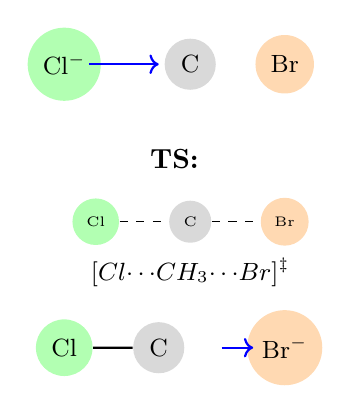
\begin{tikzpicture}[scale=0.8]
% Reactants
\node[circle,fill=green!30,minimum size=0.5cm] (Cl) at (0,2) {\small Cl$^-$};
\node[circle,fill=gray!30,minimum size=0.5cm] (C) at (2,2) {\small C};
\node[circle,fill=orange!30,minimum size=0.5cm] (Br) at (3.5,2) {\small Br};
\draw[->,thick,blue] (0.4,2) -- (1.5,2);
% TS
\node at (1.75,0.5) {\textbf{TS:}};
\node[circle,fill=green!30,minimum size=0.4cm] (Cl2) at (0.5,-0.5) {\tiny Cl};
\node[circle,fill=gray!30,minimum size=0.4cm] (C2) at (2,-0.5) {\tiny C};
\node[circle,fill=orange!30,minimum size=0.4cm] (Br2) at (3.5,-0.5) {\tiny Br};
\draw[dashed] (Cl2) -- (C2);
\draw[dashed] (C2) -- (Br2);
\node at (2,-1.3) {\small $[Cl{\cdots}CH_3{\cdots}Br]^\ddagger$};
% Products
\node[circle,fill=green!30,minimum size=0.5cm] (Cl3) at (0,-2.5) {\small Cl};
\node[circle,fill=gray!30,minimum size=0.5cm] (C3) at (1.5,-2.5) {\small C};
\node[circle,fill=orange!30,minimum size=0.5cm] (Br3) at (3.5,-2.5) {\small Br$^-$};
\draw[thick] (Cl3) -- (C3);
\draw[->,thick,blue] (2.5,-2.5) -- (3.0,-2.5);
\end{tikzpicture}
\end{column}
\end{columns}
\end{frame}

\begin{frame}{Case Study 2: E2 Elimination}
\begin{columns}
\begin{column}{0.55\textwidth}
\centering
\includegraphics[width=\textwidth]{E2.png}
\end{column}
\begin{column}{0.42\textwidth}
\textbf{E2 elimination:}
\begin{itemize}
\item Concerted: base removes $\beta$-H while leaving group departs
\item Anti-periplanar geometry required
\item One TS, no intermediate
\end{itemize}

\vspace{0.5em}
\textbf{Competition with S\textsubscript{N}2:}
\begin{itemize}
\item Same reactants, different TS
\item $\Delta\Delta G^\ddagger$ determines selectivity
\item Strong base + bulky substrate $\rightarrow$ E2
\item Good nucleophile + primary substrate $\rightarrow$ S\textsubscript{N}2
\end{itemize}
\end{column}
\end{columns}
\end{frame}

\begin{frame}{Case Study 3: Diels--Alder Cycloaddition}
\[
\text{Butadiene} + \text{Ethene} \xrightarrow{\Delta} \text{Cyclohexene}
\]

\vspace{0.5em}
\begin{columns}
\begin{column}{0.55\textwidth}
\textbf{Key features:}
\begin{itemize}
\item [4+2] cycloaddition -- concerted, pericyclic
\item Two new C--C bonds form simultaneously
\item TS is \emphr{aromatic} (6 electrons in cyclic array)
\item Highly ordered TS $\Rightarrow$ $\Delta S^\ddagger \ll 0$
\end{itemize}

\vspace{0.5em}
\textbf{DFT results} (B3LYP-D3/6-311+G(d,p)):
\begin{itemize}
\item $\Delta E^\ddagger \approx 22$ kcal/mol
\item $\Delta H^\ddagger \approx 20$ kcal/mol (ZPE correction)
\item $\Delta G^\ddagger \approx 33$ kcal/mol (large $-T\Delta S^\ddagger$!)
\item $\Delta G_\text{rxn} \approx -38$ kcal/mol
\end{itemize}
\end{column}
\begin{column}{0.42\textwidth}
\centering
\begin{tikzpicture}[scale=0.9]
\draw[->] (0,0) -- (6,0) node[right] {\small Rxn coord.};
\draw[->] (0,0) -- (0,4.5) node[above] {\small $\Delta G$};
% Reactant
\draw[thick,blue,smooth] plot coordinates {(0.5,2.5) (1,2) (1.5,2.5)};
% TS
\draw[thick,blue,smooth] plot coordinates {(1.5,2.5) (2,3) (2.5,3.8) (3,4.2) (3.5,3.8) (4,3)};
% Product
\draw[thick,blue,smooth] plot coordinates {(4,3) (4.5,1.5) (5,0.5) (5.5,1)};
\node at (1,1.5) {\small R};
\node at (3,4.7) {\small TS};
\node at (5,0) {\small P};
\draw[<->,thick,red] (1.2,2) -- node[left] {\scriptsize $\Delta G^\ddagger$} (1.2,4.2);
\draw[dotted] (1,2) -- (3,2);
\draw[dotted] (1.2,4.2) -- (3,4.2);
\end{tikzpicture}

\vspace{0.3em}
\small Note: $\Delta S^\ddagger$ contributes $\sim$13 kcal/mol to the barrier at 298 K!
\end{column}
\end{columns}
\end{frame}

\begin{frame}{Case Study 4: Catalysis -- Lowering the Barrier}
\textbf{A catalyst provides an alternative pathway with a \emphr{lower barrier}:}

\vspace{0.5em}
\centering
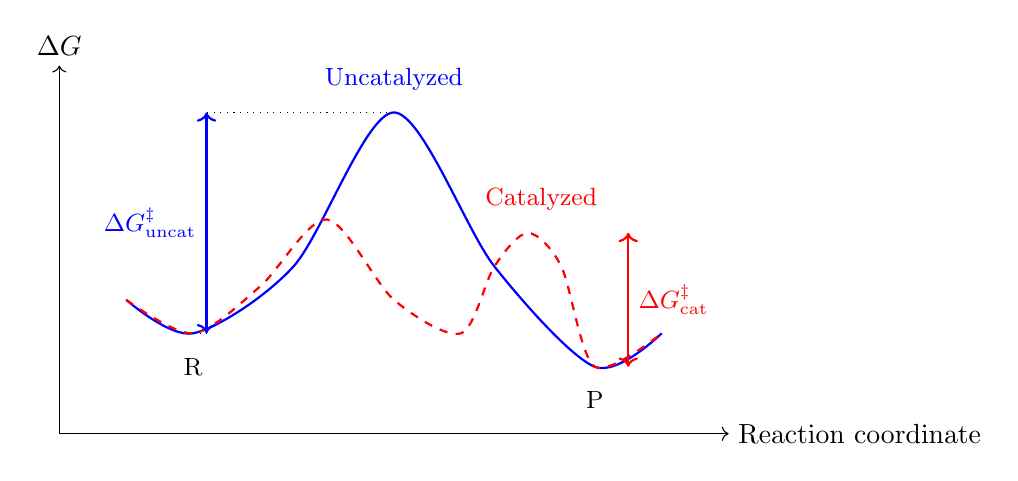
\begin{tikzpicture}[scale=0.85]
\draw[->] (0,0) -- (10,0) node[right] {Reaction coordinate};
\draw[->] (0,0) -- (0,5.5) node[above] {$\Delta G$};
% Uncatalyzed
\draw[thick,blue,smooth] plot coordinates {(1,2) (2,1.5) (3.5,2.5) (5,4.8) (6.5,2.5) (8,1.0) (9,1.5)};
% Catalyzed
\draw[thick,red,dashed,smooth] plot coordinates {(1,2) (2,1.5) (3,2.2) (4,3.2) (5,2.0) (6,1.5) (6.5,2.5) (7,3.0) (7.5,2.5) (8,1.0) (9,1.5)};
% Labels
\node[blue] at (5,5.3) {\small Uncatalyzed};
\node[red] at (7.2,3.5) {\small Catalyzed};
\node at (2,1.0) {\small R};
\node at (8,0.5) {\small P};
\draw[<->,thick,blue] (2.2,1.5) -- node[left] {\small $\Delta G^\ddagger_\text{uncat}$} (2.2,4.8);
\draw[<->,thick,red] (8.5,1.0) -- node[right] {\small $\Delta G^\ddagger_\text{cat}$} (8.5,3.0);
\draw[dotted] (2,1.5) -- (2.2,1.5);
\draw[dotted] (5,4.8) -- (2.2,4.8);
\end{tikzpicture}

\vspace{0.5em}
\begin{itemize}
\item Catalyst lowers $\Delta G^\ddagger$ but does \emphr{not} change $\Delta G_\text{rxn}$
\item DFT can map the full catalytic cycle
\item Compare barriers for catalyzed vs.\ uncatalyzed paths
\item Identify the rate-determining step in the catalytic cycle
\end{itemize}
\end{frame}


% ============================================================================
% SECTION 6: SELECTIVITY
% ============================================================================
\section{Selectivity and Competing Pathways}

\begin{frame}{Selectivity from Energy Profiles}
When multiple products are possible, \textbf{selectivity} is determined by $\Delta\Delta G^\ddagger$:

\vspace{0.5em}
\begin{columns}
\begin{column}{0.50\textwidth}
\centering
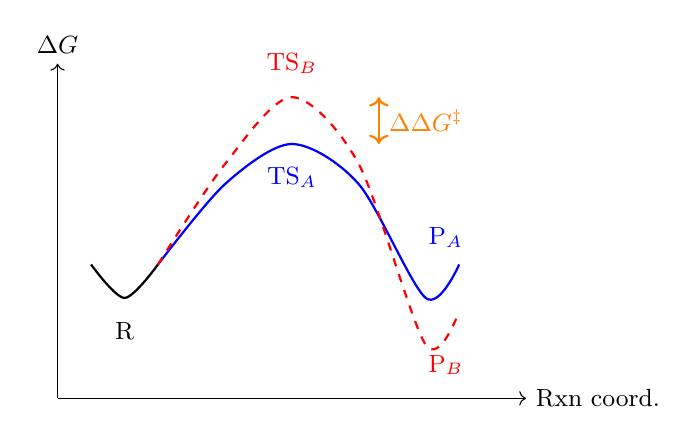
\begin{tikzpicture}[scale=0.85]
\draw[->] (0,0) -- (7,0) node[right] {\small Rxn coord.};
\draw[->] (0,0) -- (0,5) node[above] {\small $\Delta G$};
% Reactant
\draw[thick,black,smooth] plot coordinates {(0.5,2) (1,1.5) (1.5,2)};
% Path A (lower barrier)
\draw[thick,blue,smooth] plot coordinates {(1.5,2) (2.5,3.2) (3.5,3.8) (4.5,3.2) (5.5,1.5) (6,2)};
% Path B (higher barrier)
\draw[thick,red,dashed,smooth] plot coordinates {(1.5,2) (2.5,3.5) (3.5,4.5) (4.5,3.5) (5.5,0.8) (6,1.3)};
\node at (1,1.0) {\small R};
\node[blue] at (3.5,3.3) {\small TS$_A$};
\node[red] at (3.5,5.0) {\small TS$_B$};
\node[blue] at (5.8,2.4) {\small P$_A$};
\node[red] at (5.8,0.5) {\small P$_B$};
\draw[<->,thick,orange] (4.8,3.8) -- node[right] {\small $\Delta\Delta G^\ddagger$} (4.8,4.5);
\end{tikzpicture}
\end{column}
\begin{column}{0.48\textwidth}
\textbf{Kinetic selectivity:}
\[
\frac{k_A}{k_B} = \e^{-\Delta\Delta G^\ddagger / RT}
\]

At 298 K:
\begin{center}
\begin{tabular}{cc}
\toprule
$\Delta\Delta G^\ddagger$ & Selectivity \\
\midrule
0.5 kcal/mol & 70:30 \\
1.0 kcal/mol & 84:16 \\
1.4 kcal/mol & 90:10 \\
2.0 kcal/mol & 97:3 \\
3.0 kcal/mol & 99.4:0.6 \\
\bottomrule
\end{tabular}
\end{center}
\end{column}
\end{columns}

\vspace{0.3em}
\textbf{Note:} Product $B$ is more stable (thermodynamic product) but Product $A$ forms faster (kinetic product). \emphr{Kinetic vs.\ thermodynamic control!}
\end{frame}

\begin{frame}{Thermodynamic vs.\ Kinetic Control}
\begin{columns}
\begin{column}{0.55\textwidth}
\textbf{Kinetic control} (low $T$, short time):
\begin{itemize}
\item Product formed \emphr{fastest} dominates
\item Determined by $\Delta G^\ddagger$ (barrier height)
\item Irreversible conditions
\end{itemize}

\vspace{0.5em}
\textbf{Thermodynamic control} (high $T$, long time):
\begin{itemize}
\item Most \emphr{stable} product dominates
\item Determined by $\Delta G_\text{rxn}$ (reaction free energy)
\item Reversible conditions (equilibrium)
\end{itemize}

\vspace{0.5em}
\textbf{Boltzmann distribution at equilibrium:}
\[
\frac{N_A}{N_B} = \e^{-(G_A - G_B)/RT}
\]
\end{column}
\begin{column}{0.42\textwidth}
\centering
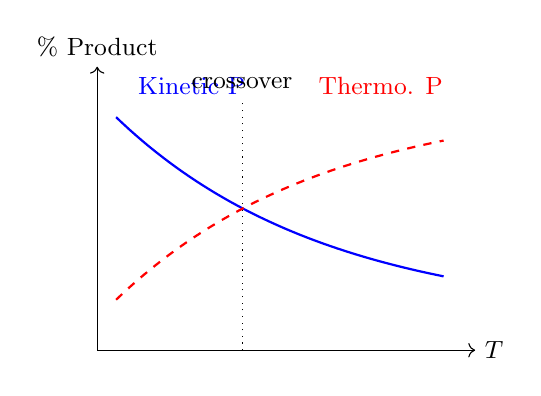
\begin{tikzpicture}[scale=0.8]
\draw[->] (0,0) -- (6,0) node[right] {\small $T$};
\draw[->] (0,0) -- (0,4.5) node[above] {\small \% Product};
% Kinetic product
\draw[thick,blue,domain=0.3:5.5,samples=50] plot (\x, {3.5*exp(-0.3*\x) + 0.5});
% Thermodynamic product
\draw[thick,red,dashed,domain=0.3:5.5,samples=50] plot (\x, {4 - 3.5*exp(-0.3*\x)});
\node[blue] at (1.5,4.2) {\small Kinetic P};
\node[red] at (4.5,4.2) {\small Thermo. P};
\draw[dotted] (2.3,0) -- (2.3,4) node[above] {\small crossover};
\end{tikzpicture}

\vspace{0.5em}
\small At low $T$: kinetic product dominates.\\
At high $T$: thermodynamic product dominates.
\end{column}
\end{columns}
\end{frame}

\begin{frame}{Regioselectivity Example: Electrophilic Aromatic Substitution}
\textbf{Nitration of toluene:} Where does \ch{NO2+} attack?

\vspace{0.5em}
\begin{center}
\begin{tabular}{lccc}
\toprule
\textbf{Position} & $\Delta G^\ddagger$ (kcal/mol) & \textbf{Relative rate} & \textbf{Product \%} \\
\midrule
\textit{ortho} & 21.5 & 1.0 & $\sim$58\% \\
\textit{meta} & 23.8 & 0.02 & $\sim$4\% \\
\textit{para} & 21.8 & 0.6 & $\sim$37\% \\
\bottomrule
\end{tabular}
\end{center}

\vspace{0.5em}
\textbf{DFT can predict:}
\begin{itemize}
\item Activation barriers for each regioisomeric pathway
\item Product ratios from $\Delta\Delta G^\ddagger$
\item Effect of substituents on selectivity
\item Statistical corrections for equivalent positions (\textit{ortho}: $\times 2$, \textit{para}: $\times 1$)
\end{itemize}
\end{frame}

\begin{frame}{Stereoselectivity -- Enantioselective Catalysis}
\textbf{DFT can predict enantioselectivity} by comparing TS energies for R and S products:

\vspace{0.5em}
\[
\text{ee} = \frac{|k_R - k_S|}{k_R + k_S} \times 100\% = \frac{|\e^{-\Delta G_R^\ddagger/RT} - \e^{-\Delta G_S^\ddagger/RT}|}{\e^{-\Delta G_R^\ddagger/RT} + \e^{-\Delta G_S^\ddagger/RT}} \times 100\%
\]

\vspace{0.5em}
\begin{center}
\begin{tabular}{cc}
\toprule
$\Delta\Delta G^\ddagger_{R/S}$ (kcal/mol) & \textbf{ee (\%)} \\
\midrule
0.5 & 40 \\
1.0 & 70 \\
1.4 & 84 \\
2.0 & 93 \\
3.0 & 99 \\
\bottomrule
\end{tabular}
\end{center}

\vspace{0.3em}
\emphr{Just 2 kcal/mol} difference gives $>$90\% ee!\\
This is within DFT accuracy -- predictions are meaningful but require careful methodology.
\end{frame}


% ============================================================================
% SECTION 7: PRACTICAL CONSIDERATIONS
% ============================================================================
\section{Practical Considerations}

\begin{frame}{Choosing the Right Level of Theory for Reactions}
\begin{center}
\begin{tabular}{lp{4cm}l}
\toprule
\textbf{Level} & \textbf{Good for} & \textbf{Typical error} \\
\midrule
B3LYP/6-31G(d) & Quick screening, qualitative trends & 3--5 kcal/mol \\
B3LYP-D3/def2-TZVP & Organic reactions, conformational analysis & 2--3 kcal/mol \\
$\omega$B97X-D/def2-TZVP & General purpose, thermochemistry & 1--3 kcal/mol \\
PBE0-D3/def2-TZVP & Transition metals, organometallics & 2--4 kcal/mol \\
DLPNO-CCSD(T)/cc-pVTZ & ``Gold standard'' single points & $<$1 kcal/mol \\
\bottomrule
\end{tabular}
\end{center}

\vspace{0.5em}
\textbf{Common strategy:} Optimize at DFT, single-point at CCSD(T)
\begin{itemize}
\item Geometry: B3LYP-D3/def2-TZVP (cheap, geometries are good)
\item Energy: DLPNO-CCSD(T)/cc-pVTZ//B3LYP-D3/def2-TZVP
\item Thermal corrections: from the DFT frequency calculation
\end{itemize}
\end{frame}

\begin{frame}{Solvent Effects}
\textbf{Many reactions occur in solution}, not gas phase!

\vspace{0.5em}
\textbf{Implicit solvation models} (continuum):
\begin{itemize}
\item \textbf{PCM} (Polarizable Continuum Model) -- Gaussian default
\item \textbf{SMD} (Solvation Model based on Density) -- recommended for $\Delta G_\text{solv}$
\item \textbf{COSMO/CPCM} -- ORCA, Turbomole
\end{itemize}

\vspace{0.5em}
\textbf{Effect on barriers:}
\begin{itemize}
\item Charged species are strongly stabilized in polar solvents
\item S\textsubscript{N}1: solvent stabilizes carbocation $\Rightarrow$ \emphr{lowers} barrier
\item S\textsubscript{N}2: solvent stabilizes nucleophile more than TS $\Rightarrow$ \emphr{raises} barrier
\item Neutral reactions: smaller solvent effects
\end{itemize}

\vspace{0.5em}
In Gaussian: \texttt{SCRF=(SMD,Solvent=Water)}\\
In ORCA: \texttt{! CPCM(Water)}
\end{frame}

\begin{frame}{Dispersion Corrections -- Don't Forget Them!}
\textbf{Standard DFT functionals miss London dispersion forces:}
\begin{itemize}
\item Attractive van der Waals interactions between all atoms
\item Crucial for: conformational energies, reaction barriers involving large molecules, non-covalent interactions
\end{itemize}

\vspace{0.5em}
\textbf{Popular dispersion corrections:}
\begin{center}
\begin{tabular}{lll}
\toprule
\textbf{Method} & \textbf{Type} & \textbf{Key features} \\
\midrule
DFT-D3 (Grimme) & Pairwise additive & BJ or zero damping; most common \\
DFT-D4 (Grimme) & Charge-dependent & Improved over D3 \\
XDM (Johnson) & Dipole moment model & Non-empirical; my research area! \\
VV10/NL & Nonlocal functional & Self-consistent; no atom parameters \\
\bottomrule
\end{tabular}
\end{center}

\vspace{0.5em}
\textbf{Rule of thumb:} \emphr{Always} use dispersion corrections unless you have a good reason not to.\\
In Gaussian: \texttt{B3LYP/def2-TZVP EmpiricalDispersion=GD3BJ}
\end{frame}

\begin{frame}{Common Pitfalls in Reaction Modeling}
\begin{enumerate}
\item \textbf{Not verifying the TS}
\begin{itemize}
\item Always check: 1 imaginary frequency + IRC
\end{itemize}

\item \textbf{Comparing energies at different levels of theory}
\begin{itemize}
\item All species must use the same method/basis set
\end{itemize}

\item \textbf{Forgetting thermal corrections}
\begin{itemize}
\item $\Delta E \neq \Delta G$! Use $\Delta G$ for rate constants
\end{itemize}

\item \textbf{Ignoring conformational sampling}
\begin{itemize}
\item The lowest-energy conformer matters; check multiple conformers
\end{itemize}

\item \textbf{Missing solvent effects}
\begin{itemize}
\item Gas-phase barriers can differ by $>$10 kcal/mol from solution
\end{itemize}

\item \textbf{Low-frequency mode errors}
\begin{itemize}
\item Modes $< 100$ cm$^{-1}$ cause large errors in $S_\text{vib}$ and $G$
\item Use Grimme's quasi-RRHO or Truhlar's quasi-harmonic correction
\end{itemize}

\item \textbf{Neglecting dispersion}
\begin{itemize}
\item Use D3, D4, or XDM corrections with your functional
\end{itemize}
\end{enumerate}
\end{frame}


% ============================================================================
% SECTION 8: COMPUTATIONAL WORKFLOW
% ============================================================================
\section{Computational Workflow}

\begin{frame}{Complete Workflow: Studying a Reaction with DFT}
\begin{center}
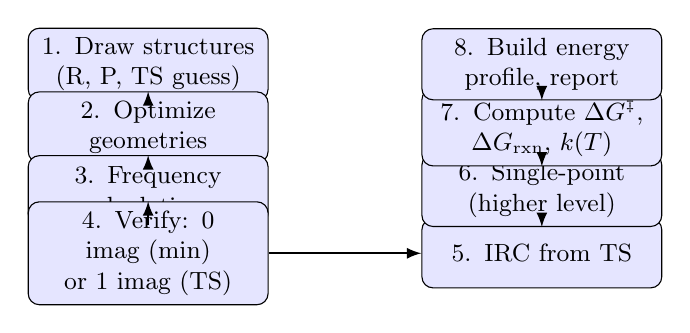
\begin{tikzpicture}[node distance=0.8cm, auto,
    block/.style={rectangle, draw, fill=blue!10, text width=8em, text centered, rounded corners, minimum height=2.5em, font=\small},
    line/.style={draw, -latex, thick}]

    \node [block] (draw) {1. Draw structures\\(R, P, TS guess)};
    \node [block, below of=draw] (opt) {2. Optimize\\geometries};
    \node [block, below of=opt] (freq) {3. Frequency\\calculations};
    \node [block, below of=freq] (check) {4. Verify: 0 imag (min)\\ or 1 imag (TS)};
    \node [block, right of=check, node distance=5cm] (irc) {5. IRC from TS};
    \node [block, above of=irc] (sp) {6. Single-point\\(higher level)};
    \node [block, above of=sp] (thermo) {7. Compute $\Delta G^\ddagger$,\\$\Delta G_\text{rxn}$, $k(T)$};
    \node [block, above of=thermo] (report) {8. Build energy\\profile, report};

    \path [line] (draw) -- (opt);
    \path [line] (opt) -- (freq);
    \path [line] (freq) -- (check);
    \path [line] (check) -- (irc);
    \path [line] (irc) -- (sp);
    \path [line] (sp) -- (thermo);
    \path [line] (thermo) -- (report);
\end{tikzpicture}
\end{center}
\end{frame}

\begin{frame}[fragile]{Example ORCA Input: TS Optimization}
\begin{tcolorbox}[colback=snow,colframe=charcoal,fontupper=\ttfamily\scriptsize,title={\texttt{ts\_opt.inp}}]
\begin{verbatim}
! B3LYP D3BJ def2-TZVP OptTS Freq
%maxcore 4000
%pal nprocs 8 end

* xyz 0 1
C   0.000000   0.000000   0.000000
H   0.000000   0.000000   1.089000
H   1.026720   0.000000  -0.363000
H  -0.513360  -0.889165  -0.363000
Cl -0.513360   0.889165  -2.500000
Br  0.513360  -0.889165   2.800000
*
\end{verbatim}
\end{tcolorbox}

\vspace{0.3em}
\textbf{Key options:}
\begin{itemize}
\item \texttt{OptTS}: TS optimization using eigenvector following
\item \texttt{Freq}: frequency calculation to verify the TS
\item \texttt{D3BJ}: Grimme's D3 dispersion with Becke--Johnson damping
\end{itemize}
\end{frame}

\begin{frame}[fragile]{Example Gaussian Input: Complete Reaction Study}
\begin{tcolorbox}[colback=snow,colframe=charcoal,fontupper=\ttfamily\scriptsize,title=Step 1: Optimize Reactant]
\#p B3LYP/def2-TZVP EmpiricalDispersion=GD3BJ Opt Freq SCRF=(SMD{,}Solvent=Water)

Reactant optimization --- 0 1 --- {[}coordinates{]}
\end{tcolorbox}

\begin{tcolorbox}[colback=snow,colframe=charcoal,fontupper=\ttfamily\scriptsize,title=Step 2: Optimize TS]
\#p B3LYP/def2-TZVP EmpiricalDispersion=GD3BJ Opt=(TS{,}CalcFC{,}NoEigenTest) Freq SCRF=(SMD{,}Solvent=Water)

TS optimization --- 0 1 --- {[}coordinates from scan or QST{]}
\end{tcolorbox}

\begin{tcolorbox}[colback=snow,colframe=charcoal,fontupper=\ttfamily\scriptsize,title=Step 3: IRC]
\#p B3LYP/def2-TZVP EmpiricalDispersion=GD3BJ IRC=(CalcFC{,}MaxPoints=50{,}StepSize=10)

IRC from TS --- 0 1 --- {[}coordinates from optimized TS{]}
\end{tcolorbox}
\end{frame}


% ============================================================================
% SECTION 9: ADVANCED TOPICS
% ============================================================================
\section{Advanced Topics}

\begin{frame}{Beyond TST: Quantum Tunneling}
\textbf{TST assumes classical nuclear motion} -- but quantum effects matter!

\vspace{0.5em}
\textbf{Quantum tunneling:}
\begin{itemize}
\item Light atoms (especially H) can \emphr{tunnel through} the barrier
\item Rate is \emphr{faster} than TST prediction
\item Important for H-transfer reactions at low temperatures
\item Large kinetic isotope effects (KIE): $k_H/k_D \gg 7$
\end{itemize}

\vspace{0.5em}
\textbf{Simple corrections:}
\begin{itemize}
\item \textbf{Wigner correction:} $\kappa_W = 1 + \frac{1}{24}\left(\frac{h|\nu^\ddagger|}{k_BT}\right)^2$
\item \textbf{Eckart barrier:} fits a 1D potential to reactant, TS, product energies
\item For accurate tunneling: need multidimensional approaches (SCT, CVT/SCT)
\end{itemize}

\vspace{0.5em}
\small Example: H-atom transfer in methylhydroxycarbene $\rightarrow$ acetaldehyde occurs entirely by tunneling below 20 K!
\end{frame}

\begin{frame}{Kinetic Isotope Effects (KIE)}
\textbf{Replacing H with D changes the rate} -- a powerful mechanistic tool:

\[
\text{KIE} = \frac{k_H}{k_D}
\]

\vspace{0.5em}
\textbf{Primary KIE} (bond to H/D is broken in the RDS):
\begin{itemize}
\item $k_H/k_D \approx 2\text{--}7$ (classical, from $\Delta$ZPE)
\item $k_H/k_D > 7$: suggests tunneling contribution
\item DFT prediction: compute $\Delta G^\ddagger$ with H and with D
\end{itemize}

\vspace{0.5em}
\textbf{Secondary KIE} (bond to H/D is \emphr{not} broken):
\begin{itemize}
\item $k_H/k_D \approx 0.8\text{--}1.2$
\item Reflects changes in hybridization at the TS
\end{itemize}

\vspace{0.5em}
\textbf{DFT can predict KIE:} Run frequency calculations with different isotopic masses $\rightarrow$ different ZPE and vibrational partition functions $\rightarrow$ different $\Delta G^\ddagger$.
\end{frame}

\begin{frame}{Conformational Searching and Boltzmann Averaging}
\textbf{Problem:} Flexible molecules have many conformers. Which one do you use?

\vspace{0.5em}
\textbf{Answer:} All of them! Boltzmann-weighted average:
\[
\langle A \rangle = \frac{\sum_i A_i \,\e^{-G_i/RT}}{\sum_i \e^{-G_i/RT}}
\]

\vspace{0.5em}
\textbf{Practical approach:}
\begin{enumerate}
\item Generate conformers (CREST, RDKit, systematic search)
\item Pre-screen at low level (GFN2-xTB, PM7)
\item Optimize unique low-energy conformers at DFT level
\item Compute $\Delta G$ for each conformer
\item Boltzmann-weight to get ensemble properties
\end{enumerate}

\vspace{0.5em}
\textbf{For TS:} You need to search conformational space for the TS too!\\
Missing a lower-energy TS conformer $\Rightarrow$ overestimate the barrier.
\end{frame}


% ============================================================================
% SUMMARY
% ============================================================================
\section{Summary}

\begin{frame}{Summary of Lecture 2}
\begin{enumerate}
\item \textbf{Transition states} are first-order saddle points with exactly \emphr{one imaginary frequency}
\item \textbf{Eyring equation:} $k(T) = \frac{k_BT}{h}\e^{-\Delta G^\ddagger / RT}$ connects PES to rate constants
\item \textbf{Finding TS:} Relaxed scan $\rightarrow$ QST2/3 or NEB $\rightarrow$ eigenvector following $\rightarrow$ verify!
\item \textbf{Always verify:} 1 imaginary frequency + IRC in both directions
\item \textbf{Selectivity:} $\Delta\Delta G^\ddagger$ of $\sim$2 kcal/mol $\Rightarrow$ $>$95\% selectivity
\item \textbf{Practical:}
\begin{itemize}
\item Use dispersion corrections (D3/D4/XDM)
\item Include solvent effects (SMD/PCM)
\item Report $\Delta G$, not $\Delta E$ -- thermal corrections matter!
\item Apply quasi-RRHO for low-frequency modes
\end{itemize}
\end{enumerate}
\end{frame}

\begin{frame}{The Big Picture: DFT for Reaction Chemistry}
\centering
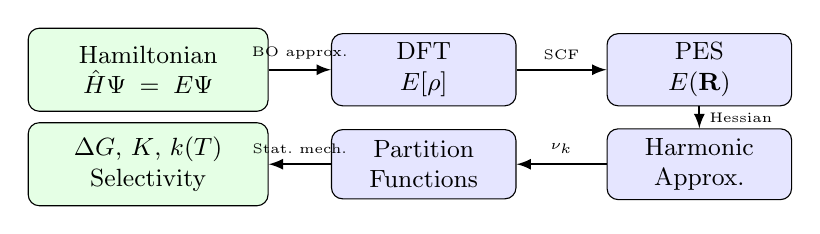
\begin{tikzpicture}[node distance=1.2cm, auto,
    block/.style={rectangle, draw, fill=blue!10, text width=6em, text centered, rounded corners, minimum height=2.5em, font=\small},
    bigblock/.style={rectangle, draw, fill=green!10, text width=8em, text centered, rounded corners, minimum height=3em, font=\small},
    line/.style={draw, -latex, thick}]

    \node [bigblock] (ham) {Hamiltonian\\$\hat{H}\Psi = E\Psi$};
    \node [block, right of=ham, node distance=3.5cm] (dft) {DFT\\$E[\rho]$};
    \node [block, right of=dft, node distance=3.5cm] (pes) {PES\\$E(\mathbf{R})$};
    \node [block, below of=pes] (harm) {Harmonic\\Approx.};
    \node [block, left of=harm, node distance=3.5cm] (part) {Partition\\Functions};
    \node [bigblock, left of=part, node distance=3.5cm] (thermo) {$\Delta G$, $K$, $k(T)$\\Selectivity};

    \path [line] (ham) -- node[above] {\tiny BO approx.} (dft);
    \path [line] (dft) -- node[above] {\tiny SCF} (pes);
    \path [line] (pes) -- node[right] {\tiny Hessian} (harm);
    \path [line] (harm) -- node[above] {\tiny $\nu_k$} (part);
    \path [line] (part) -- node[above] {\tiny Stat.\ mech.} (thermo);
\end{tikzpicture}

\vspace{1.5em}
\textbf{From first principles to chemical predictions:}\\
No empirical parameters needed (beyond the choice of functional)!\\

\vspace{0.5em}
\textit{This is the power of modern computational chemistry.}
\end{frame}

\begin{frame}{Key Equations to Remember}
\begin{columns}
\begin{column}{0.48\textwidth}
\textbf{Transition State Theory:}
\begin{align*}
k(T) &= \frac{k_BT}{h}\e^{-\Delta G^\ddagger/RT} \\[6pt]
\Delta G^\ddagger &= G(\text{TS}) - G(\text{R}) \\[6pt]
E_a &\approx \Delta H^\ddagger + RT
\end{align*}

\textbf{Selectivity:}
\[
\frac{k_A}{k_B} = \e^{-\Delta\Delta G^\ddagger / RT}
\]
\end{column}
\begin{column}{0.48\textwidth}
\textbf{TS Characterization:}
\begin{itemize}
\item $\nabla E = \mathbf{0}$
\item Exactly 1 imaginary frequency
\item IRC connects R $\leftrightarrow$ P
\end{itemize}

\vspace{0.5em}
\textbf{Free Energy:}
\[
G = E_\text{elec} + E_\text{ZPE} + H_\text{th} - TS
\]

\textbf{Equilibrium:}
\[
K = \e^{-\Delta G^\circ / RT}
\]
\end{column}
\end{columns}
\end{frame}

\begin{frame}{}
\centering
\vspace{2em}
{\LARGE \textbf{Thank you!}}

\vspace{2em}
{\large Questions?}

\vspace{2em}
\textbf{Alastair J. Price}\\
Guest Lecturer, CHM328H1 S\\
University of Toronto -- Winter 2026

\vspace{1em}
\small \textit{These lectures covered:}\\
\small 1. DFT foundations: Hamiltonian $\rightarrow$ KS-DFT $\rightarrow$ PES $\rightarrow$ Harmonic approx.\ $\rightarrow$ Thermodynamics\\
\small 2. Reactions: Transition states $\rightarrow$ Eyring equation $\rightarrow$ Energy profiles $\rightarrow$ Selectivity
\end{frame}

% ============================================================================
% OPTIONAL BUFFER SLIDES (47-53)
% Use if time permits
% ============================================================================

\begin{frame}{Numerical Example -- S$_N$2 Reaction (Eyring Calculation)}
\small
Reaction: Cl$^-$ + CH$_3$Br $\rightarrow$ CH$_3$Cl + Br$^-$

\vspace{0.3em}
\textbf{DFT Results (B3LYP/6-31+G*):}
\begin{itemize}
\item Electronic barrier: $\Delta E^\ddagger \approx 5$ kcal/mol
\item Free energy barrier: $\Delta G^\ddagger \approx 23$ kcal/mol at 298 K
\end{itemize}

\vspace{0.3em}
\textbf{Eyring Equation:} $k(T) = \kappa \cdot \frac{k_B T}{h} \cdot \exp\left(\frac{-\Delta G^\ddagger}{RT}\right)$

\vspace{0.3em}
At 298 K with $\Delta G^\ddagger = 23$ kcal/mol:
\begin{itemize}
\item Pre-exponential: $\frac{k_B T}{h} \approx 6.2 \times 10^{12}$ s$^{-1}$
\item Exponential: $\exp(-23/RT) \approx 1.4 \times 10^{-17}$
\item \textbf{Result:} $k \approx 8.4 \times 10^{-5}$ s$^{-1}$ (slow in gas phase)
\end{itemize}

Note: Two molecules combining causes large entropy penalty ($\sim 18$ kcal/mol).
\end{frame}

\begin{frame}{Numerical Example -- Diels--Alder (Entropy Effects)}
\small
Reaction: C$_4$H$_6$ + C$_2$H$_4$ $\rightarrow$ C$_6$H$_{10}$ (cyclohexene)

\vspace{0.3em}
\textbf{Experimental barrier:} $\sim 27$ kcal/mol | \textbf{DFT (B3LYP):} $\sim 24$ kcal/mol

\vspace{0.3em}
\textbf{Energy Breakdown:}
\begin{itemize}
\item Electronic: $\Delta E^\ddagger \approx 22$ kcal/mol
\item ZPE: $+0.5$ kcal/mol
\item Thermal: $+0.2$ kcal/mol
\item \textbf{Entropy:} $\Delta S^\ddagger \approx -45$ J/(mol·K) $\Rightarrow$ $T\Delta S^\ddagger \approx -13.4$ kcal/mol
\end{itemize}

\vspace{0.2em}
Therefore: $\Delta G^\ddagger = 22 + 0.2 - (-13.4) \approx 35.6$ kcal/mol

\textbf{Key insight:} Entropy accounts for $\sim 13$ kcal/mol! Electronic energy alone is not predictive.
\end{frame}

\begin{frame}{Numerical Example -- Unimolecular Isomerization}
\small
Reaction: HCN $\rightarrow$ HNC (isomerization)

\vspace{0.3em}
\textbf{Experimental barrier:} $11.6 \pm 0.2$ kcal/mol | \textbf{DFT:} $10.8$--$12.0$ kcal/mol

\vspace{0.3em}
\textbf{Energy Breakdown:}
\begin{itemize}
\item Electronic: $\Delta E^\ddagger \approx 10.8$ kcal/mol
\item ZPE + Thermal: $\sim 0.4$ kcal/mol
\item Entropy: $\Delta S^\ddagger \approx +5$ J/(mol·K) $\Rightarrow$ negligible
\end{itemize}

\vspace{0.2em}
Therefore: $\Delta G^\ddagger \approx \Delta E^\ddagger$ (they're nearly equal!)

\vspace{0.2em}
\textbf{Eyring:} $k \approx 6.2 \times 10^{12} \times \exp(-10.8/RT) \approx 6.8 \times 10^4$ s$^{-1}$

\textbf{Comparison:} Unimolecular ($6.8 \times 10^4$ s$^{-1}$) vs. bimolecular ($8.4 \times 10^{-5}$ s$^{-1}$) $\Rightarrow$ entropy penalty is huge!
\end{frame}

\begin{frame}{Entropy Comparison: Unimolecular vs.\ Bimolecular}
\small
\centering
\begin{tabular}{lccc}
\toprule
\textbf{Reaction Type} & $\Delta S^\ddagger$ & \textbf{Effect} & \textbf{Example} \\
\midrule
Unimolecular & $\approx 0$ & Minimal & Isomerization \\
Bimolecular & $-40$ to $-60$ J/(mol·K) & Raises $\Delta G^\ddagger$ by 10--15 kcal/mol & S$_N$2, D--A \\
Dissociative & $+40$ to $+60$ J/(mol·K) & Lowers $\Delta G^\ddagger$ by 10--15 kcal/mol & Bond homolysis \\
\bottomrule
\end{tabular}

\vspace{0.5em}
At 298 K, $T\Delta S^\ddagger$ ranges from $-14$ kcal/mol to $+14$ kcal/mol.

\vspace{0.3em}
\textbf{Implications:}
\begin{itemize}
\item S$_N$2 is slow in gas phase but fast in solution
\item Diels--Alder barriers are $\sim 10$ kcal/mol higher than electronic energy
\item Some reactions reverse at high $T$ (entropy-driven)
\end{itemize}

\textbf{Moral:} ALWAYS compute $\Delta G$, not $\Delta E$.
\end{frame}

\begin{frame}{Method Selection Decision Tree}
\small
\textbf{Quick screening?} $\rightarrow$ B3LYP/6-31G(d) or GFN2-xTB (error: 3--5 kcal/mol)

\vspace{0.2em}
\textbf{Standard organic chemistry?} $\rightarrow$ B3LYP-D3/def2-TZVP or PBE-D3/def2-TZVP (error: 2--3 kcal/mol)

\vspace{0.2em}
\textbf{Charge transfer or long-range?} $\rightarrow$ $\omega$B97X-D/def2-TZVP or CAM-B3LYP-D3 (error: 1--2 kcal/mol)

\vspace{0.2em}
\textbf{Enantioselectivity or high accuracy?} $\rightarrow$ DFT geometry + CCSD(T) single-point (error: $<1$ kcal/mol)

\vspace{0.2em}
\textbf{Large molecules?} $\rightarrow$ B3LYP-D3/6-31G(d) geometry, then B3LYP-D3/def2-TZVP single-point

\vspace{0.3em}
\textbf{ALWAYS:}
\begin{itemize}
\item Add dispersion (D3/D4/XDM)
\item Include solvent (PCM or SMD)
\item Verify TS: exactly one imaginary frequency
\item Run IRC in both directions
\end{itemize}
\end{frame}

\begin{frame}{Pitfall: Missing IRC Verification}
\small
\textbf{What went wrong?} Found a structure with exactly one imaginary frequency, declared it a TS. But IRC didn't connect to the expected product.

\vspace{0.3em}
\textbf{What happened?} The structure was a saddle point, but not the correct TS:
\begin{itemize}
\item Maybe it's a TS for a different pathway
\item Maybe it's a competing reaction
\item Maybe it's a higher-order saddle point with a very small second frequency
\end{itemize}

\vspace{0.3em}
\textbf{The fix:}
\begin{enumerate}
\item Always run IRC in BOTH directions (forward and backward)
\item Forward direction MUST end at products (same atoms, same connectivity)
\item Backward direction MUST end at reactants
\item If IRC doesn't reach expected structures: the TS is wrong
\end{enumerate}

\textbf{Why it matters:} Without IRC, you don't know what reaction you're studying!

\textbf{Cost-benefit:} IRC takes 5 minutes, saves hours of confusion.
\end{frame}

\begin{frame}{Pitfall: Ignoring Solvent in Ionic Reactions}
\small
\textbf{What went wrong?} Computed S$_N$2 barrier in gas phase: $\Delta G^\ddagger \approx 23$ kcal/mol $\Rightarrow$ $k \approx 10^{-5}$ s$^{-1}$. Experiment in solution: $\sim 10^3$ s$^{-1}$ (six orders of magnitude faster!).

\vspace{0.3em}
\textbf{What happened?} In gas phase, the TS is highly polar (two negative charges). DFT doesn't stabilize this. In solution, the solvent dramatically stabilizes the charged TS, lowering $\Delta G^\ddagger$ by 8--10 kcal/mol.

\vspace{0.2em}
Corrected: $\Delta G^\ddagger(\text{solvent}) \approx 23 - 9 = 14$ kcal/mol

Eyring: $k \approx 10^3$ s$^{-1}$ (matches experiment!)

\vspace{0.3em}
\textbf{The fix:}
\begin{enumerate}
\item For ANY reaction with charged species: ADD SOLVENT
\item Use implicit solvation (PCM or SMD in Gaussian/ORCA)
\item Aqueous: \texttt{solvent=water}; Organic: \texttt{solvent=acetonitrile}
\item Recompute TS and check $\Delta G^\ddagger$ (often 5--15 kcal/mol lower)
\end{enumerate}

\textbf{Solvent effects are not small.} They're often larger than differences between good and bad methods.
\end{frame}

\end{document}
